In this section, we will go in into some of the implementation details of our math tutoring conversational agent. Specifically, we will discuss the data and architecture we have decided on using.

\subsection{Data}
\label{Data}
To be able to recognize the users' affective behaviour we used a pre-trained model\footnote{https://github.com/atulapra/Emotion-detection} that takes visual input using a camera, converts it to a 48x48 grayscale image and uses that to classify a range of 7 different emotions. The input is not saved during or after the emotion detection to make sure we don't harm the privacy of the user. We do not ask the user for any personal data for the same reason, as it is not required to teach math skill. Although we acknowledge that it could make the interactions more personalized.

\subsection{Architecture}
\label{Architecture}
Our bot is entirely built on an interaction framework called Furhat \cite{Furhat}; it provides extensive documentation and functionalities including gaze behaviour, gesturing, speech profiles, and more.\\

\noindent Furhat is mainly based on finite state transitions, so our systems architecture uses a rule-based approach to dialogue management. This design decision was mainly based on the robustness requirement we had for the bot, as the task can be modelled using a finite amount of states and we would like to stay in control of the tutor as to make sure the goal of the conversation is reached. Our dialogue flow is modelled in a UML format and can be found in appendix \ref{appendix:a}.\\

\noindent To make sure our conversational agent also has adaptive behaviour when it comes to both verbal and non-verbal input, we took a different approach than the rule-based one. As mentioned in the previous section we used machine learning principles instead, a convolutional neural network to be exact. The neural network classifies user emotion using visual input of the face of the user in real-time. These classified emotions are in turn used to determine the best approach in gazing, gesturing and even dialogue decisions to make sure the user has a constructive learning experience. In the figures below two examples are presented, showing the facial recognition and emotion classification in two different scenarios.

\begin{figure}[h]
\centering
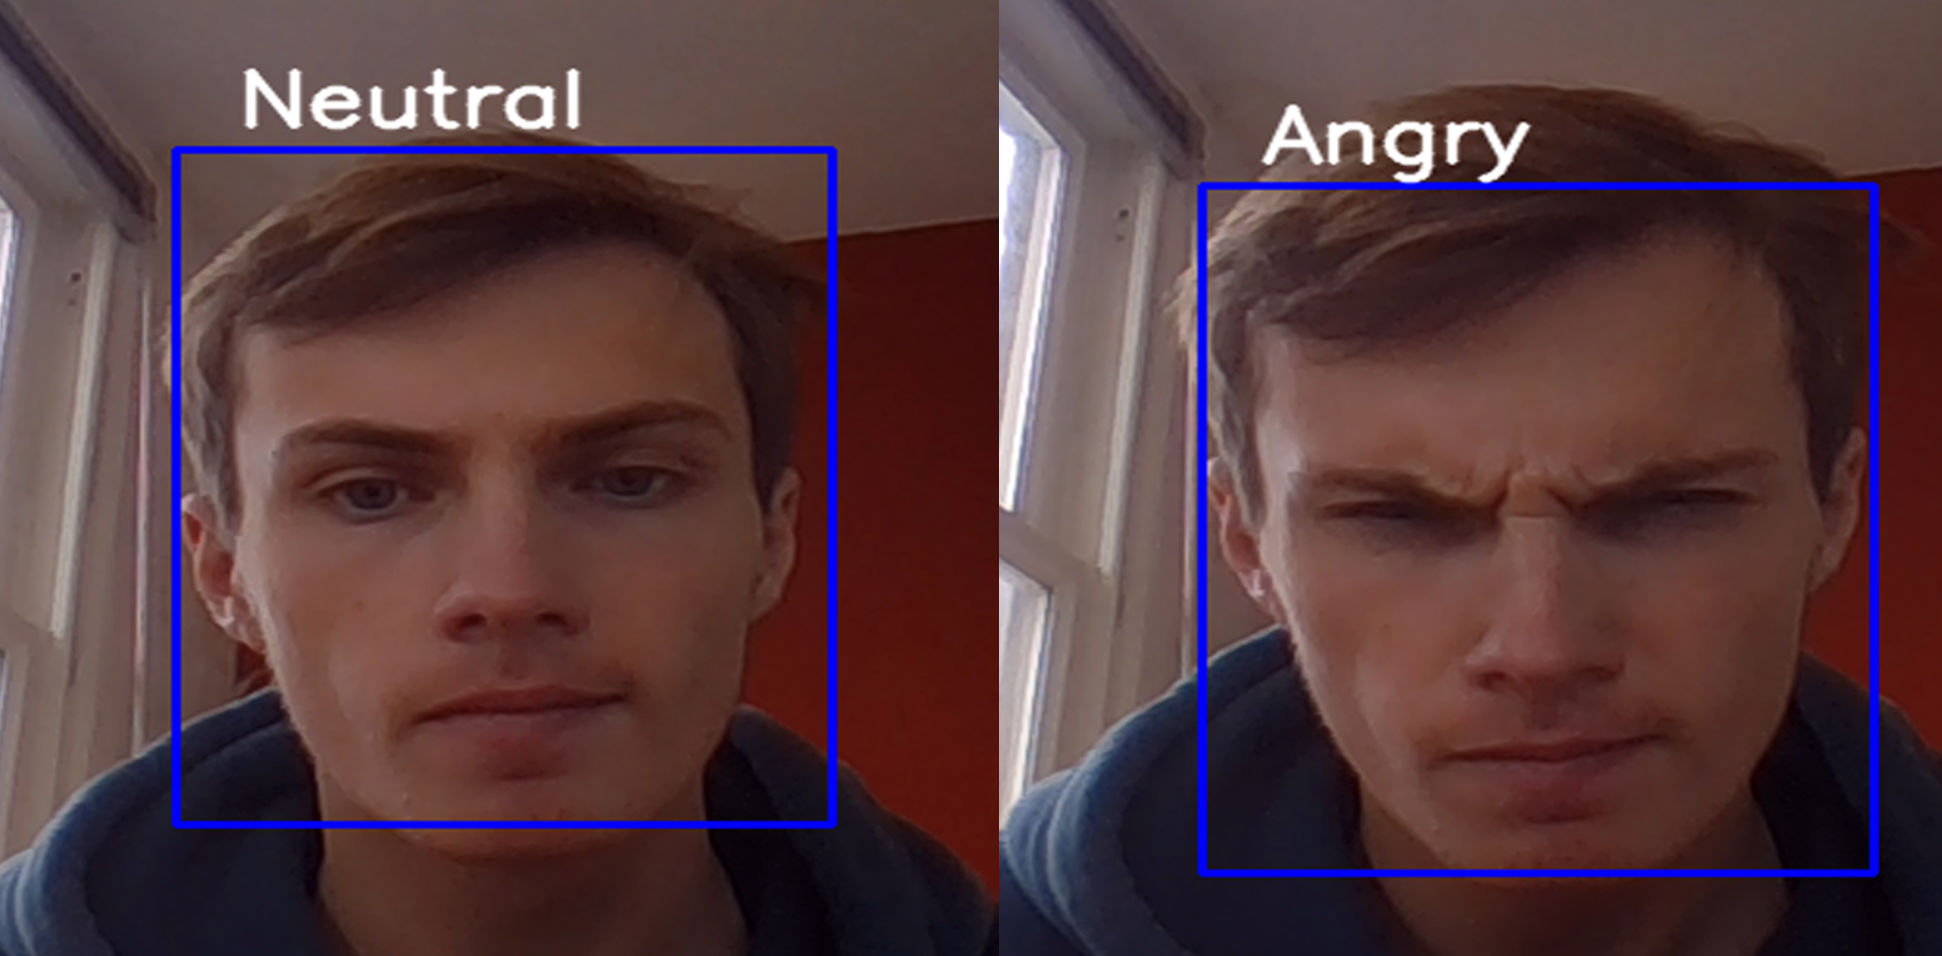
\includegraphics[width=\linewidth]{images/neutral_angry.png}
\caption{The classification of two affective behaviours}
\label{fig:emotion_detection}
\end{figure}

\subsection{Dialog flow}
The dialogue flow that we implemented for our agent can be found in appendix A. To create it we just imagined what a standard math teaching routine is like, and came up with dialogue lines that the tutor would say in that scenario. We separated them into 3 files in our project structure. The introduction and encouragement based on emotions are in mathtutor.kt, the explanations with examples are in explanation.kt, and the exercise questions (including generation) are in exercises.kt. We thought the agent was speaking a bit too fast during the explanations, so we changed the voice rate during those utterances to be 0.7. The agent has multiple possible lines it can say to encourage the user based on the detected emotion, and it randomly picks one of them each time it tries to encourage the user. This adds some variety to the dialogue and makes the agent seem more human-like. 

\subsection{Gaze behavior}
There are 3 types of gaze behavior which we could have implemented for our agent: random, rule-based, and data-driven. We immediately ruled out random because it would obviously be unreliable and probably very annoying from the user's perspective. In the end, we chose to use rule-based gaze behavior because it is much simpler to implement than creating a data-driven model, while it still achieves the desired effects with the right rules.
\newline
\newline
The two main gaze rules that we implemented are based on a research paper about the functions of gaze direction \cite{kendon1967some}. First, at the beginning of a long utterance, the agent should look away from the user. This gives the impression that the agent is still formulating the rest of what it is going to say. At the end of the utterance, it should look right at the user because it expects a response or reaction from the user. To implement this we made our agent look away for a few seconds at the start of long utterances and then look at the user after that. The location at which it looks away is chosen randomly from 4 points (up-left, up-right, down-left, down-right). We put extra pauses in the explanations during which the virtual agent glances away from the user as if the agent is preparing the next part of the explanation. When the agent continues, it just looks at the user again.
\newline
\newline
The other main rule we used is that the agent should look a bit lower than eye contact at the user for the beginning of long utterances, and end up looking into the users' eyes. To implement this rule we made it such that when our agent looks at the user during explanations, it looks slightly downwards, until asking the user for confirmation if they understood the explanation. For both of these rules we assume that the user is centered in front of the screen, at the same height as the agent. We had to use this assumption because we could not find where to get the location of the current user in Furhat.
\subsection{Gestures}
Gestures can potentially make the agent seem more human and we believe that will improve the user experience. That's why we decided to add some simple gesture behavior to the agent. By default, it wears a friendly smile towards the user. When the agent confirms an answer from the user to be correct it will put on a bigger smile and nod. If the user gives a wrong answer the agent will put away the smile while trying to console/encourage the user to make sure it is not perceived as laughing at the user for getting it wrong. After the exercise session, if the user got at least 60\% correct, it will show a bigger smile to them, then stop smiling after a second and ask the user if they want to practice more or not. If the user asks for help during the exercise session the agent will nod at them to confirm that it is going to help them.


\subsection{Emotion Detection}
The detect of emotion is very crucial when it comes in conversations involving humans interacting with humans. Many times, humans detect the emotions of the other speakers and intuitively they change their behaviour according to other's speaker feelings in order not to make them feel uncomfortable. Let's say that in a conversation between humans, one of them makes an inappropriate comment against the other and the other person feels sad. Then the person making the comment realizes that he said something wrong by seeing him sad, and feels sorry about it so he asks for forgiveness. Thus,  emotion detection is an essential part of our lives and plays a crucial role in how a conversation progresses.
\newline
\newline
Taking into consideration everything that has been said, it is evident that is very important for a conversational agent to be able to capture the emotions of the user to have a real conversation. The script that was used to detect the emotion of the user, is written in python using the pre-trained model which was mentioned in section \ref{Data}. The classes of the pre-trained model are 7: \{Angry, Disgusted, Happy, Neutral, Sad, Fearful, Surprised\}. Then, after the emotion has been detected, it is sent to a web-server (localhost:5000) where our agent parses the result and "combines" it with the user responses to give its reply. Therefore, each time the agent needs to know the emotion of the user, it will make a request to the web-server. The web-server calls the Emotion Detection script to capture the user's face at that moment and outputs the detected emotion on the web-server. This output is then processed by the agent. It should be noted that an assumption has been made that when the program cannot detect any face the moment it was requested, it always returns Neutral. 

\subsection{Usage of Emotion Detector}
The emotion detector was mostly used during the explanations of the math skill (e.g. percentages), as we want to detect if the user understands the explanation given by the agent. The agent will comfort the user if needed. It will do so based on the users' utterances and detected emotion. 
For the same reasons, the emotion was also captured in states where the exercises are being provided and explained.
\newline
\newline
Let's consider as an example the state Explanation1 to get a feeling of how the emotion detection works in combination with the user's responses. Firstly, the agent starts by requesting the users' emotion and if it detects surprise \textbf{before} starting the explanation, it will gon on encouraging the user before continuing with the explanation. When the explanation is completed, the agent asks whether the student has understood the given explanation. If the user responses "Yes" or "No" it transitions to the next states \textbf{without} checking his emotions. We have chosen this because the agents' main priority should be what the user said, regardless of what emotion has been detected. This is done for two reasons. Firstly, in real life, people tend to rely more on what the speaker is saying as this conveys more information and your detected emotion could be misjudged. Secondly, our emotion detector is not accurate enough to confidently rely on the detected emotion. 
If a user requests a "Repeat", the agent will detect the user's emotion and gives a motivational speech based on the detected emotion. Similarly, if a user responds with "do not know" or "do not understand", the agent detects the emotion and moves to the appropriate state. A diagram of this process is shown in appendix \ref{appendix:a}.